\documentclass[12pt]{article}
\usepackage{tikz}
\usepackage[margin=0.1in]{geometry}

\begin{document}

\begin{center}
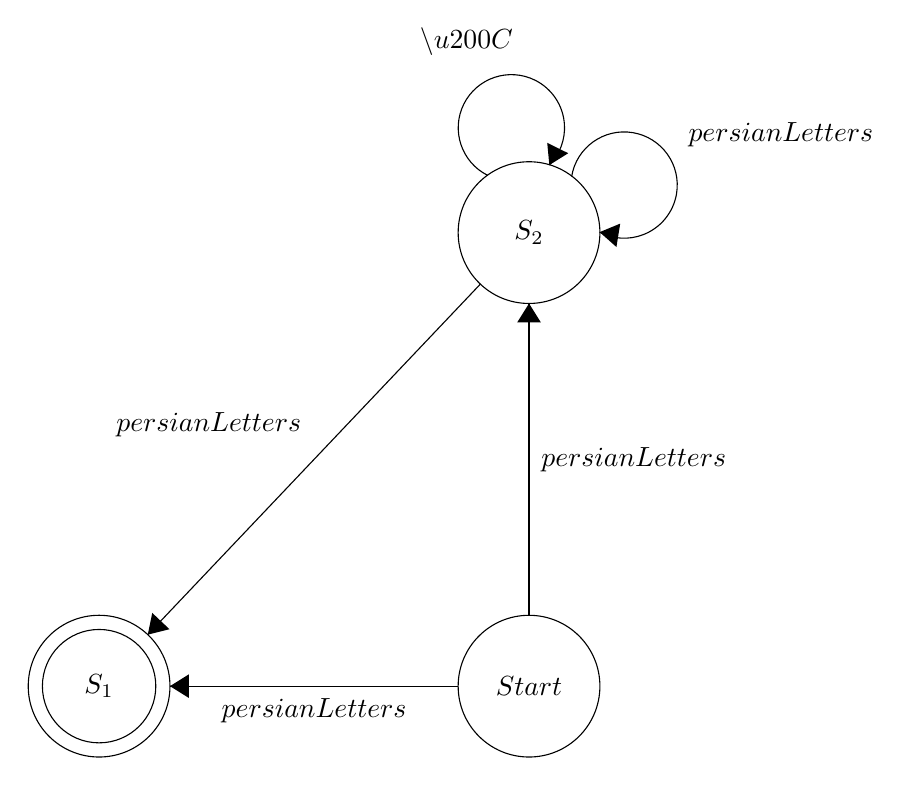
\begin{tikzpicture}[scale=0.3]
\tikzstyle{every node}+=[inner sep=0pt]
\draw [black] (39.2,-37) circle (3);
\draw (39.2,-37) node {$Start$};
\draw [black] (21,-37) circle (3);
\draw (21,-37) node {$S_1$};
\draw [black] (21,-37) circle (2.4);
\draw [black] (39.2,-17.8) circle (3);
\draw (39.2,-17.8) node {$S_2$};
\draw [black] (36.2,-37) -- (24,-37);
\fill [black] (24,-37) -- (24.8,-37.5) -- (24.8,-36.5);
\draw (30.1,-37.5) node [below] {$persianLetters$};
\draw [black] (39.2,-34) -- (39.2,-20.8);
\fill [black] (39.2,-20.8) -- (38.7,-21.6) -- (39.7,-21.6);
\draw (39.7,-27.4) node [right] {$persianLetters$};
\draw [black] (37.451,-15.377) arc (243.55484:-44.44516:2.25);
\draw (36.55,-10.32) node [above] {$\texttt{\textbackslash}u200C$};
\fill [black] (40.06,-14.94) -- (40.86,-14.44) -- (39.97,-14);
\draw [black] (41.005,-15.419) arc (170.56505:-117.43495:2.25);
\draw (45.93,-13.67) node [right] {$persianLetters$};
\fill [black] (42.19,-17.78) -- (42.9,-18.41) -- (43.06,-17.42);
\draw [black] (37.14,-19.98) -- (23.06,-34.82);
\fill [black] (23.06,-34.82) -- (23.98,-34.59) -- (23.25,-33.9);
\draw (29.57,-25.93) node [left] {$persianLetters$};
\end{tikzpicture}
\end{center}

\end{document}
